%%%%%%%%%%%%%%%%%%%%%%%%%%%%%%%%%%%%%%%%%%%%%%%%%%%%%%%%%%%%
%%  This Beamer template was created by Cameron Bracken.
%%  Anyone can freely use or modify it for any purpose
%%  without attribution.
%%
%%  Last Modified: January 9, 2009
%%

\documentclass[xcolor=x11names,compress]{beamer}
\usepackage[utf8]{inputenc}
\usepackage[french]{babel}
\usepackage{lmodern}
\usepackage{amsmath}
\usepackage{amsfonts}
%% General document %%%%%%%%%%%%%%%%%%%%%%%%%%%%%%%%%%
\usepackage{graphicx}
\usepackage{caption}
\usepackage{subcaption}
\usepackage{tikz}
\usetikzlibrary{decorations.fractals}
	\usepackage{multimedia}
	\usepackage{media9}
%%%%%%%%%%%%%%%%%%%%%%%%%%%%%%%%%%%%%%%%%%%%%%%%%%%%%%


%% Beamer Layout %%%%%%%%%%%%%%%%%%%%%%%%%%%%%%%%%%
\useoutertheme[subsection=false,shadow]{miniframes}
\useinnertheme{default}
\usefonttheme{serif}
\usepackage{palatino}

\setbeamerfont{title like}{shape=\scshape}
\setbeamerfont{frametitle}{shape=\scshape}

\setbeamercolor*{lower separation line head}{bg=DeepSkyBlue4} 
\setbeamercolor*{normal text}{fg=black,bg=white} 
\setbeamercolor*{alerted text}{fg=red} 
\setbeamercolor*{example text}{fg=black} 
\setbeamercolor*{structure}{fg=black} 
 
\setbeamercolor*{palette tertiary}{fg=black,bg=black!10} 
\setbeamercolor*{palette quaternary}{fg=black,bg=black!10} 

\renewcommand{\(}{\begin{columns}}
\renewcommand{\)}{\end{columns}}
\newcommand{\<}[1]{\begin{column}{#1}}
\renewcommand{\>}{\end{column}}
%%%%%%%%%%%%%%%%%%%%%%%%%%%%%%%%%%%%%%%%%%%%%%%%%%

\newcommand{\HRule}{\rule{\linewidth}{0.5mm}}

\addtobeamertemplate{footline}{\hspace{11cm}\large \insertframenumber/\inserttotalframenumber}


\begin{document}


%%%%%%%%%%%%%%%%%%%%%%%%%%%%%%%%%%%%%%%%%%%%%%%%%%%%%%%%%%%%%%%%%%%%%%%%%%%%%%%%%%%%%%%%%%%%%%%%%%%%%%%%%%
%---------------------------------------------------------------------------------------------------------
%%%%%%%%%%%%%%%%%%%%%%%%%%%%%%%%%%%%%%%%%%%%%%%%%%%%%%%%%%%%%%%%%%%%%%%%%%%%%%%%%%%%%%%%%%%%%%%%%%%%%%%%%%


\begin{frame}
\centering
Université du Maine - Licence SPI~ 3\textsuperscript{ème} année\\
	28 mai 2014
 \vspace{1.4cm}

\HRule \\[0.6cm]
{\large \bfseries \textsc{Étude du phénomène de dispersion}  } \\[0.4cm]
\HRule \\[1.5cm]

\begin{minipage}{0.495\textwidth}
\begin{flushleft}
~\newline
 Thomas \textsc{ Lechat}\\
Alice \textsc{ Dinsenmeyer}\\
\end{flushleft}
\end{minipage}
\begin{minipage}{0.495\textwidth}
\begin{flushright} 
\emph{Encadrés par } \\
 Sohbi \textsc{ Sahraoui} \\
\small Professeur à l'université du Maine
% Supervisor's Name
\end{flushright}
\end{minipage}



\titlepage
\end{frame}

%%%%%%%%%%%%%%%%%%%%%%%%%%%%%%%%%%%%%%%%%%%%%%%%%%%%%%
%%%%%%%%%%%%%%%%%%%%%%%%%%%%%%%%%%%%%%%%%%%%%%%%%%%%%%
\begin{frame}{}
\tableofcontents
\end{frame}


%%%%%%%%%%%%%%%%%%%%%%%%%%%%%%%%%%%%%%%%%%%%%%%%%%%%%%%%%%%%%%%%%%%%%%%%%%%%%%%%%%%%%%%%%%%%%%%%%%%%%%%%%%
%---------------------------------------------------------------------------------------------------------
%%%%%%%%%%%%%%%%%%%%%%%%%%%%%%%%%%%%%%%%%%%%%%%%%%%%%%%%%%%%%%%%%%%%%%%%%%%%%%%%%%%%%%%%%%%%%%%%%%%%%%%%%%
\section{\scshape Dans les milieux continus}
\subsection{Dispersion dans un guide d'onde}
\begin{frame}{}


{\scshape Dans les milieux continus}
\begin{itemize}
	\item[]Dispersion dans un guide d'onde
\end{itemize}
\end{frame}

%%%%%%%%%%%%%%%%%%%%%%%%%%%%%%%%%%%%%%%%%%%%%%%%%%%%%%
%%%%%%%%%%%%%%%%%%%%%%%%%%%%%%%%%%%%%%%%%%%%%%%%%%%%%%

\begin{frame}{Mise en équation de la pression}
	\begin{itemize}
		\item Équation de propagation : 
		\begin{equation*}
			\nabla^2p - \frac{1}{c^2}\frac{\partial{^2p}}{\partial{t}^2} = 0 \qquad \text{avec} \qquad p(x,y,t) = X(x)Y(y)T(t)
		\end{equation*}
		
		\item Solution de cette équation :
		\begin{itemize}
			\item $Y(y) = A\cos{k_yy}+B\sin{k_yy}$
			\item $X(x) = Ce^{-jk_xx}$
			\item $T(t) = e^{~j\omega t}$ 
		\end{itemize}
		\bigskip
		d'où : 
		\begin{equation}
			p(x,y,t) = [A\cos{k_yy}+B\sin{k_yy}]Ce^{-jk_xx} e^{~jwt}
		\end{equation}
	\end{itemize} 

\end{frame}

%%%%%%%%%%%%%%%%%%%%%%%%%%%%%%%%%%%%%%%%%%%%%%%%%%%%%%
%%%%%%%%%%%%%%%%%%%%%%%%%%%%%%%%%%%%%%%%%%%%%%%%%%%%%%

\begin{frame}{Application des conditions limites à la paroi}
	\begin{itemize}
		\item Paroi infiniment rigide : 
		\begin{equation*}
			\left.\frac{\partial{p}}{\partial{y}}\right|_{\begin{smallmatrix}y=0 \\ y=L\end{smallmatrix}} = 0 \qquad \Rightarrow \qquad \begin{cases} B = 0 \\ k_{yn} = \frac{n\pi}{L} \end{cases}
		\end{equation*}		
		\item Finalement :
		\begin{equation}
				p(x,y,t) = \sum_n A_n \cos\left(\frac{n\pi}{L}y\right)e^{-jk_{xn}x}e^{~j\omega t}
			\end{equation}
		\bigskip
		avec : 
		\begin{equation}
			k_{xn} =\sqrt{k^2-k_{yn}^2}= \sqrt{k^2-\left(\frac{n\pi}{L}\right)^2}
		\end{equation}
	\end{itemize} 

\end{frame}

%%%%%%%%%%%%%%%%%%%%%%%%%%%%%%%%%%%%%%%%%%%%%%%%%%%%%%
%%%%%%%%%%%%%%%%%%%%%%%%%%%%%%%%%%%%%%%%%%%%%%%%%%%%%%
%\subsection{Vitesse de phase}
\begin{frame}{Vitesse de phase}
	Définie par : 
	\begin{equation}
		c_{ph_n} = \frac{\omega}{k_{xn}} = \frac{c}{\sqrt{1-\left(\frac{n\pi}{kL}\right)^2}}
	\end{equation}
	\bigskip
	\begin{figure}
		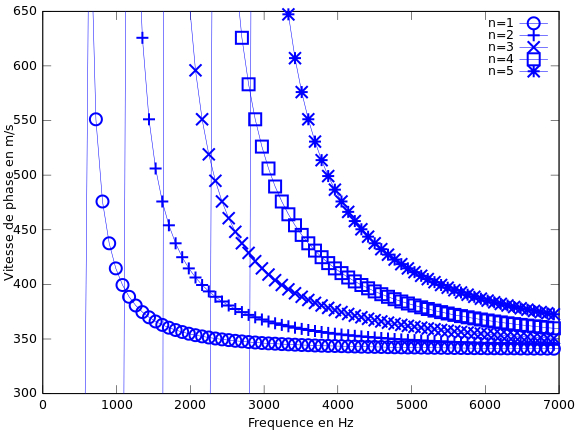
\includegraphics[scale=0.35]{./figures/c_phase.jpg}
		\caption*{\scriptsize Vitesse de phase en fonction de la fréquence, pour les 5 premiers modes (L = 30 cm, c = 340 m/s).}
	\end{figure}
\end{frame}


%%%%%%%%%%%%%%%%%%%%%%%%%%%%%%%%%%%%%%%%%%%%%%%%%%%%%%
%%%%%%%%%%%%%%%%%%%%%%%%%%%%%%%%%%%%%%%%%%%%%%%%%%%%%%
%\subsection{Vitesse de groupe}
\begin{frame}{Vitesse de groupe}
Définie par : 
	\begin{equation}
		c_{gn} = \frac{\mathrm{d}\omega}{\mathrm{d}k_{xn}} = c\sqrt{1-\left(\frac{n\pi}{kL}\right)^{2}}
	\end{equation}
	\bigskip
	\begin{figure}
		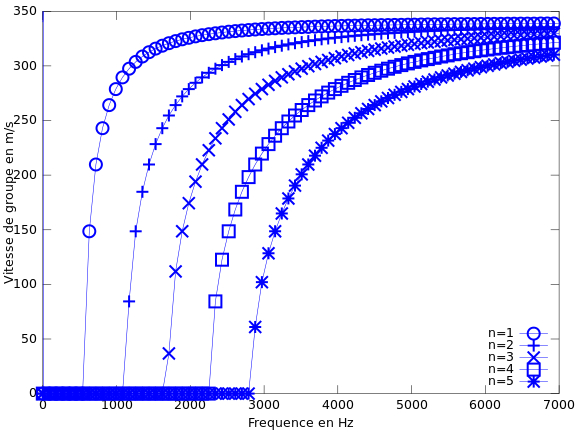
\includegraphics[scale=0.35]{./figures/c_groupe.jpg}
		\caption*{\scriptsize Vitesse de groupe en fonction de la fréquence, pour les 5 premiers modes (L = 30 cm, c = 340 m/s).}
	\end{figure}

\end{frame}


%%%%%%%%%%%%%%%%%%%%%%%%%%%%%%%%%%%%%%%%%%%%%%%%%%%%%%
%%%%%%%%%%%%%%%%%%%%%%%%%%%%%%%%%%%%%%%%%%%%%%%%%%%%%%
\begin{frame}{Visualisation de la vitesse de groupe}
	\begin{eqnarray*}
		\begin{cases}
			p_1 = A\cos(\omega_1t-k_1x) \\
			p_2 = A\cos(\omega_2t-k_2x)
		\end{cases}  
	\end{eqnarray*}
	\bigskip
	\begin{equation}
		 \Rightarrow  p_1+p_2 =2A\cos\left(\Delta \omega t-\Delta kx\right)\cos\left(\omega_0 t-k_0x\right)
	\end{equation}
	\bigskip
avec
\scriptsize
\begin{equation*}
\Delta \omega = \frac{\omega_1-\omega_2}{2} \qquad \text{,~} \qquad \Delta k = \frac{k_1-k_2}{2} \qquad \text{,~} \qquad  \omega_0 = \frac{\omega_1+\omega_2}{2} \qquad \text{ et } \qquad  k_0 = \frac{k_1+k_2}{2}
\end{equation*}

\begin{center}
\bigskip
\bigskip
	\boxed {
\href{moire_dispersion.avi}{Video} } 
\end{center} 
\end{frame}


%%%%%%%%%%%%%%%%%%%%%%%%%%%%%%%%%%%%%%%%%%%%%%%%%%%%%%%%%%%%%%%%%%%%%%%%%%%%%%%%%%%%%%%%%%%%%%%%%%%%%%%%%%
%---------------------------------------------------------------------------------------------------------
%%%%%%%%%%%%%%%%%%%%%%%%%%%%%%%%%%%%%%%%%%%%%%%%%%%%%%%%%%%%%%%%%%%%%%%%%%%%%%%%%%%%%%%%%%%%%%%%%%%%%%%%%%

\subsection{Dispersion dans une poutre en flexion}
\begin{frame}{}


{\scshape Dans les milieux continus}
\begin{itemize}
	\item[]Vibration d'une poutre encastrée-libre en flexion
\end{itemize}
\end{frame}

\begin{frame}{Schéma de la poutre}

\begin{figure}[!h]
\centering{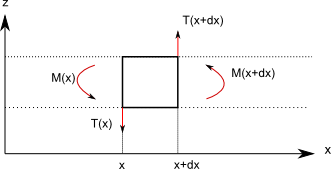
\includegraphics[scale=0.7]{./figures/segment_poutre.png}}
\caption*{ \scriptsize Forces s’exerçant sur un élément de longueur $dx$ d'une poutre en flexion}
\end{figure}

On utilise les approximations suivantes:
\begin{itemize}
\item  $M(x+dx) = M(x) + \frac{\partial M(x)}{\partial x} dx$   
\item $T(x+dx) = T(x) + \frac{\partial T(x)}{\partial x} dx$
\end{itemize}
\end{frame}

%%%%%%%%%%%%%%%%%%%%%%%%%%%%%%%%%%%%%%%%%%%%%%%%%%%%%%
%%%%%%%%%%%%%%%%%%%%%%%%%%%%%%%%%%%%%%%%%%%%%%%%%%%%%%
%\subsection{Application du principe fondamentale de la dynamique}
\begin{frame}{}

On applique le PFD à un élément de poutre de longueur $dx$:
\begin{equation}
\sum F_{ext} = \frac{\partial ^2 W}{\partial t^2} dm \qquad \Rightarrow \qquad \boxed{\frac{\partial T(x)}{\partial x} = \rho S \frac{\partial ^2 W}{\partial t^2}}
\end{equation}

Le théorème des moments donne : 
\begin{equation}
\boxed{-\frac{\partial ^2 M(x)}{\partial x^2} = \frac{\partial T(x)}{\partial x}}
\end{equation}
Enfin on peut calculer les moments dans la poutre:
\begin{eqnarray}
&&
\begin{cases}
dM(x) = z dF \Rightarrow M(x) = \int_S z dF \\
dF = -E z \frac{\partial ^2 W}{\partial x^2} dS
\end{cases} \\
 &\Rightarrow & \qquad \boxed{M(x) = -E I \frac{\partial ^2 W}{\partial x^2}}
\end{eqnarray}
%- \int_S E z^2 \frac{\partial ^2 W}{\partial x^2} dS = 
\end{frame}

%%%%%%%%%%%%%%%%%%%%%%%%%%%%%%%%%%%%%%%%%%%%%%%%%%%%%%
%%%%%%%%%%%%%%%%%%%%%%%%%%%%%%%%%%%%%%%%%%%%%%%%%%%%%%
%\subsection{Équation de propagation dans la poutre}
\begin{frame}{Équation de propagation dans la poutre}
On obtient finalement:
\begin{equation}
\rho S \frac{\partial ^2 W}{\partial t^2} = E I \frac{\partial ^4 W}{\partial x^4}
\end{equation}
On pose : $W(x,t) = f(x) g(t)$ pour résoudre cette équation. On obtient les solutions suivantes:
\begin{eqnarray*}
g(t) & = & A \cos(\omega t) + B \sin(\omega t) \\
f(x) & = & C \cos(\beta x) + D \sin(\beta x) + F \cosh(\beta x) + G \sinh(\beta x)
\end{eqnarray*}
Avec :
\begin{equation}
\beta = \sqrt[4]{\frac{\rho S \omega^2}{EI}}
\label{eq1}
\end{equation}
\end{frame}

%%%%%%%%%%%%%%%%%%%%%%%%%%%%%%%%%%%%%%%%%%%%%%%%%%%%%%
%%%%%%%%%%%%%%%%%%%%%%%%%%%%%%%%%%%%%%%%%%%%%%%%%%%%%%
%\subsection{Diagramme de dispersion}
\begin{frame}{Diagramme de dispersion}
On a:
\begin{equation}
 c_{phase} = \frac{\omega}{\beta} = \sqrt{\omega} \sqrt[4]{\frac{EI}{\rho S}}
\end{equation}
\begin{figure}[h!]
\centering 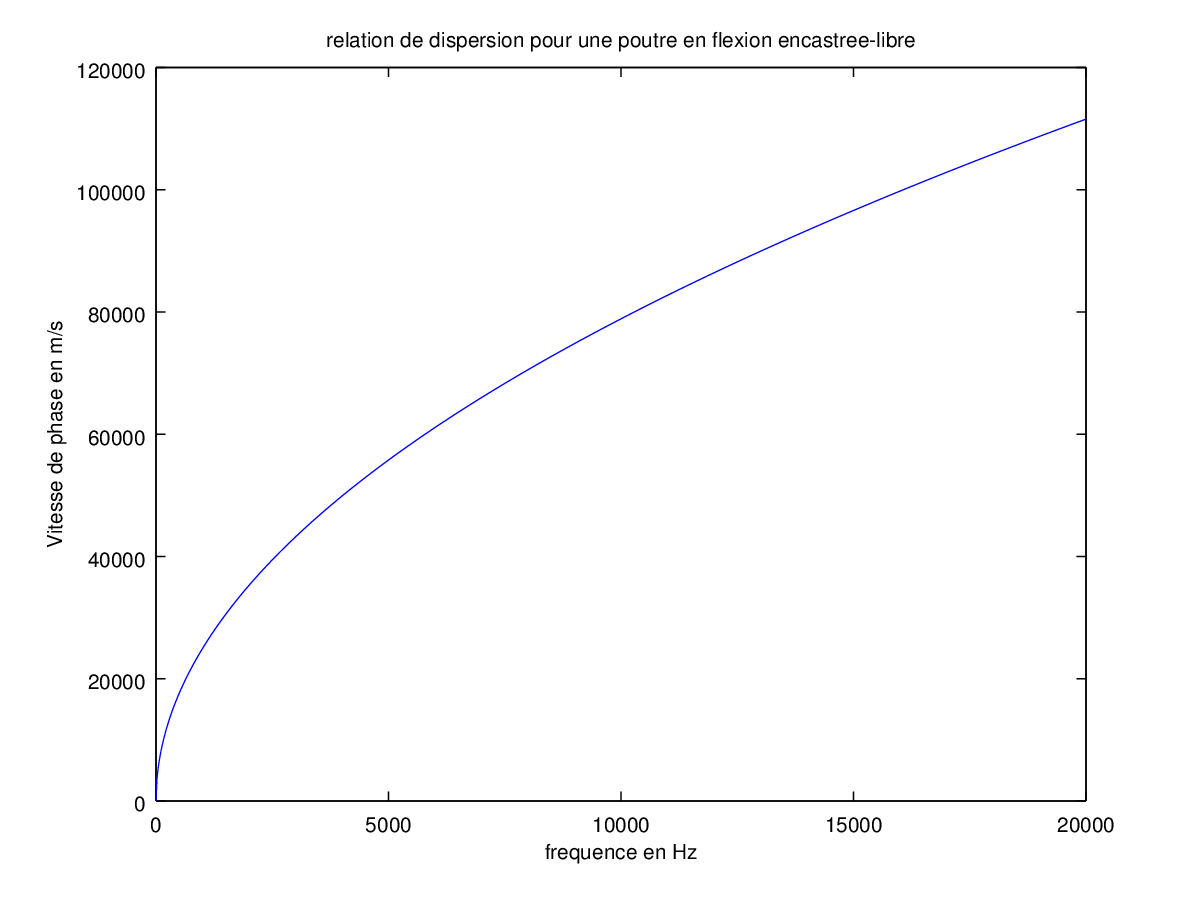
\includegraphics[scale = 0.3]{./figures/poutre_dispersion.png}
\caption*{ \scriptsize Relation de dispersion d'une poutre en acier de 3~m de longueur, 2~cm d'épaisseur et 10~cm de largeur.} \label{poutre_graphic2}
\end{figure}
\end{frame}

%%%%%%%%%%%%%%%%%%%%%%%%%%%%%%%%%%%%%%%%%%%%%%%%%%%%%%
%%%%%%%%%%%%%%%%%%%%%%%%%%%%%%%%%%%%%%%%%%%%%%%%%%%%%%
%\subsection{Application des conditions limites}
\begin{frame}{Application des conditions limites}
Poutre encastrée-libre:\\~\\

\begin{minipage}[t]{0.49\linewidth}
\begin{itemize}
	\item Encastrement:
\end{itemize} 
\begin{eqnarray*}
\begin{cases} W(0,t) = 0 \\ \frac{\partial W(0,t)}{\partial x} = 0 \end{cases}
\end{eqnarray*}
\end{minipage}
\begin{minipage}[t]{0.49\linewidth}
\begin{itemize}
	\item Libre:
\end{itemize}
\begin{eqnarray*}
\begin{cases}  EI \frac{\partial ^2 W(L,t)}{\partial ^2 x} = 0 \\ EI \frac{\partial ^3 W(L,t)}{\partial x^3} = 0 \end{cases}
\end{eqnarray*}
\end{minipage} \\ \bigskip
Ce qui permet d'aboutir à:
\begin{equation}
 \cos(\beta L) \cosh(\beta L) = -1
\end{equation}
On doit donc discrétiser pour résoudre le problème.
\end{frame}

%%%%%%%%%%%%%%%%%%%%%%%%%%%%%%%%%%%%%%%%%%%%%%%%%%%%%%
%%%%%%%%%%%%%%%%%%%%%%%%%%%%%%%%%%%%%%%%%%%%%%%%%%%%%%
%\subsection{Fréquences propres}
\begin{frame}{Pulsations propres}
En posant $\beta_n L = R_n$, on a les solutions:
\begin{equation}
\omega_n = \frac{R_n^2}{L^2} \sqrt{\frac{EI}{\rho S}}
\end{equation}

Avec:
\begin{minipage}[c]{\textwidth}
\centering
\begin{tabular}{c|c|c }
Numéro $n$ du mode  & Valeur de $R_n$ & Valeur de $R_n^2$\\\hline
0 & 1.8751 &3.5160\\
1 &  4.6941 &22.035\\
2 & 7.8547 &61.696\\ 
$\ge$ 3 & $\frac{\pi}{2}(2n-1)$ & $\frac{\pi^{2}}{4}(2n-1)^2$
\end{tabular}
\captionof*{table}{  \scriptsize Valeurs approchées de $R_n$ permettant de calculer les fréquences propres pour une poutre encastrée-libre.}
\end{minipage}
\end{frame}

%%%%%%%%%%%%%%%%%%%%%%%%%%%%%%%%%%%%%%%%%%%%%%%%%%%%%%
%%%%%%%%%%%%%%%%%%%%%%%%%%%%%%%%%%%%%%%%%%%%%%%%%%%%%%
%\subsection{Vérification expérimentale}
\begin{frame}{Vérification expérimentale}
Schéma du dispositif de mesure:
\begin{figure}
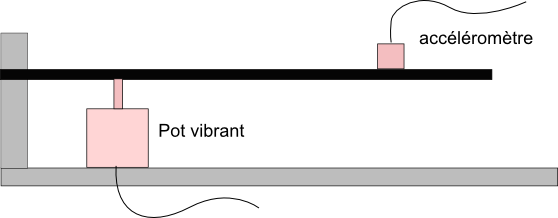
\includegraphics[scale=0.5]{./figures/presentation_poutre.png}
\caption*{\scriptsize   Schéma du dispositif de mesure}
\end{figure}
Caractéristiques de la poutre en aluminium:
\begin{itemize}
	\item masse volumique: $\rho = 2700~kg/m^3$
	\item longueur: $L = 63.5~ cm$
	\item module d'Young $E = 70~GPa$
	\item largeur $\times$ épaisseur: $30 \times 5~mm$
\end{itemize}
\end{frame}

%%%%%%%%%%%%%%%%%%%%%%%%%%%%%%%%%%%%%%%%%%%%%%%%%%%%%%
%%%%%%%%%%%%%%%%%%%%%%%%%%%%%%%%%%%%%%%%%%%%%%%%%%%%%%
%\subsection{Résultats}
\begin{frame}{Résultats}
\bigskip
\begin{minipage}[c]{\textwidth}
\centering
\begin{tabular}[0.7]{c|c|c|c }
Mode & Fréquence mesurée  & $R_n$ du mode & Valeur théorique \\\hline
0 & 9.7 Hz & 1.875 & 10.20 Hz\\
1 & 60.5 Hz & 4.694 & 63.92 Hz\\
2 & 170 Hz & 7.855 & 179.00 Hz\\
3 & 320 Hz & 10.996 & 350.00 Hz\\
4 & 707 Hz & 14.137 & 579.7 Hz 
\end{tabular}
\captionof*{table}{ \scriptsize Fréquences propres théoriques et relevées expérimentalement pour une poutre encastrée-libres.}
\end{minipage}\\~\\
Cela fonctionne bien en basses fréquences mais une erreur  se répercute en hautes fréquences.
\end{frame}


%%%%%%%%%%%%%%%%%%%%%%%%%%%%%%%%%%%%%%%%%%%%%%%%%%%%%%%%%%%%%%%%%%%%%%%%%%%%%%%%%%%%%%%%%%%%%%%%%%%%%%%%%%
%---------------------------------------------------------------------------------------------------------
%%%%%%%%%%%%%%%%%%%%%%%%%%%%%%%%%%%%%%%%%%%%%%%%%%%%%%%%%%%%%%%%%%%%%%%%%%%%%%%%%%%%%%%%%%%%%%%%%%%%%%%%%%
\section{\scshape Dans un réseau}
\subsection{Mise en équation du problème}
\begin{frame}
\large{{\scshape Dispersion dans un réseau de discontinuités}}
\end{frame}

%\subsection{mise en équation}
\begin{frame}{Équations des télégraphistes}
	\begin{minipage}[t]{0.49\linewidth}
		\begin{figure}[!h]
			\centering{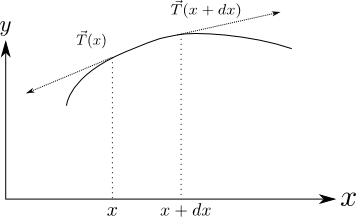
\includegraphics[scale=0.5]{./figures/schema_corde.png}}
			\caption*{\label{schema_corde} \scriptsize Schéma d'une corde vibrante sans masses ponctuelles}
		\end{figure}
	\end{minipage}
	\begin{minipage}[t]{0.49\linewidth}
		\begin{itemize}
			\item Géométrie :
			\begin{eqnarray*}
				&& \frac{T_y}{T_x} = \frac{dy}{dx} \\
				& \Rightarrow & v_y = \frac{T_y}{T_0} \\
				& \Rightarrow & \boxed{\frac{\partial v_y}{\partial x} = \frac{1}{T_0} \frac{\partial T_y}{\partial t}}
			\end{eqnarray*}
		\end{itemize}
	\end{minipage}
	\begin{itemize}
	\item PFD : 
	\begin{equation*}
		\mu dx \vec{a} (x) = \vec{T}(x) + \vec{T} (x+dx)
	\end{equation*}
	\begin{equation*}
		\left\{\begin{array}{lclcl}
			T_x (x)&=& T_x (x+dx)  &\Rightarrow &  T_x = T_0 \\
			\mu dx \frac{\partial ^2 y}{\partial t^2} &=& -T_y (x) + T_y (x+dx) &\Rightarrow &  \boxed{\mu \frac{\partial v_y}{\partial t} = \frac{\partial T_y}{\partial x}}
		\end{array}\right.
	\end{equation*}	 
\end{itemize}
\end{frame}

%%%%%%%%%%%%%%%%%%%%%%%%%%%%%%%%%%%%%%%%%%%%%%%%%%%%%%
%%%%%%%%%%%%%%%%%%%%%%%%%%%%%%%%%%%%%%%%%%%%%%%%%%%%%%

\begin{frame}{Mise sous forme matricielle}
Par séparation des variables, on a les solutions spatiales suivantes:

\begin{equation}
\begin{cases}
T(x_1)  =  A e^{-\Gamma x_1} + B e^{\Gamma x_1} \\
v(x_1)  =  -\frac{1}{j\omega\mu} [ -\Gamma A e^{-\Gamma x_1} + \Gamma B e^{\Gamma x_1}]
\end{cases}
\end{equation}
D'où la forme matricielle suivante:
\begin{eqnarray}
\begin{pmatrix} T(x_1) \\ v(x_1) \end{pmatrix} & = & \begin{pmatrix} \cos(k L) & j \sqrt{\mu T_0} \sin(k L) \\ \frac{j}{\sqrt{\mu T_0}} \sin(k L) & \cos(k L) \end{pmatrix} \begin{pmatrix} T(x_2)\\ v(x_2) \end{pmatrix} \\
& = & \begin{pmatrix} A & B \\ C & D \end{pmatrix} \begin{pmatrix} T(x_2)\\ v(x_2) \end{pmatrix}
\end{eqnarray}
Avec $\Gamma = jk = j\omega\sqrt{\frac{\mu}{T_0}}$.
\end{frame}

%%%%%%%%%%%%%%%%%%%%%%%%%%%%%%%%%%%%%%%%%%%%%%%%%%%%%%
%%%%%%%%%%%%%%%%%%%%%%%%%%%%%%%%%%%%%%%%%%%%%%%%%%%%%%
\begin{frame}{Ajout de la masse}
\begin{minipage}[t]{0.49\linewidth}
\begin{figure}[h!]
\centering 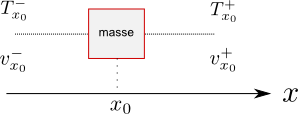
\includegraphics[scale = 0.5]{./figures/masse_graphic.png}
\caption*{\scriptsize Schéma d'un élément du réseau composé d'une masse et de 2 morceaux de corde }
\end{figure}
\end{minipage}
\begin{minipage}[t]{0.49\linewidth}
Conditions limites:
\begin{eqnarray*}
T_{x_0^{-}} = T_{x_0^{+}} + \alpha \\
v_{x_0^{-}} = v_{x_0^{+}} = v
\end{eqnarray*}
\end{minipage}

On applique le PFD à la masse:
\begin{eqnarray*}
M \frac{\partial v}{\partial t} = T_{x_0^{-}} - T_{x_0^{+}} \\
\Rightarrow T_{x_0^{-}} = j \omega M v + T_{x_0^{+}}
\end{eqnarray*} 
Finalement: 
\begin{equation}
\begin{pmatrix} T_{x_0^{-}} \\ v_{x_0^{-}} \end{pmatrix} = \begin{pmatrix} 1 & j \omega M \\ 0 & 1 \end{pmatrix}\begin{pmatrix} T_{x_0^{+}} \\ v_{x_0^{+}} \end{pmatrix}
\end{equation}
\end{frame}

%%%%%%%%%%%%%%%%%%%%%%%%%%%%%%%%%%%%%%%%%%%%%%%%%%%%%%
%%%%%%%%%%%%%%%%%%%%%%%%%%%%%%%%%%%%%%%%%%%%%%%%%%%%%%
\begin{frame}
On obtient finalement la matrice suivante pour une cellule composée d'une masse et de 2 morceaux de corde:
\begin{eqnarray*}
\begin{pmatrix} T_{x_0}^{-} \\ v_{x_0}^{-} \end{pmatrix} & = & \begin{pmatrix} A & B \\ C & D \end{pmatrix}\begin{pmatrix} 1 & j \omega M \\ 0 & 1 \end{pmatrix} \begin{pmatrix} A & B \\ C & D \end{pmatrix}  \begin{pmatrix} T_{x_0}^{+} \\ v_{x_0}^{+} \end{pmatrix} \\
& = & \begin{pmatrix} T_{11} & T_{12}\\ T_{21} & T_{22} \end{pmatrix} \begin{pmatrix} T_{x_0}^{+} \\ v_{x_0}^{+} \end{pmatrix}
\end{eqnarray*}

On a notamment:
\begin{equation}
T_{11}   = T_{22} = \cos(kd) - \frac{\omega M}{2 Zc}\sin(kd) 
\end{equation}
\end{frame}

%%%%%%%%%%%%%%%%%%%%%%%%%%%%%%%%%%%%%%%%%%%%%%%%%%%%%%
%%%%%%%%%%%%%%%%%%%%%%%%%%%%%%%%%%%%%%%%%%%%%%%%%%%%%%
\begin{frame}{Équation de dispersion}
Pour un réseau infini :
\begin{equation}
	\cos(\Gamma_{eq} d) = T_{22} = \cos(kd) - \frac{\omega M}{2 Zc}\sin(kd)
\end{equation}

\begin{figure}
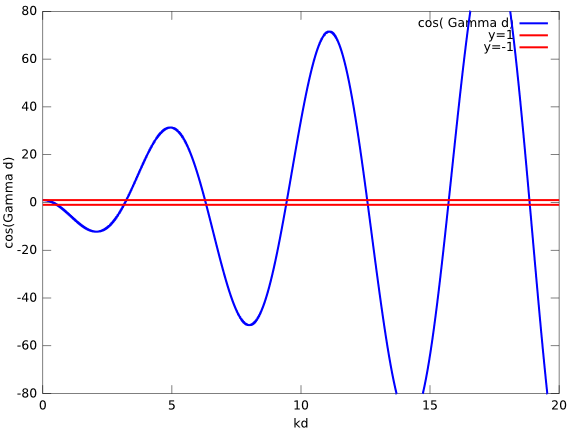
\includegraphics[scale = 0.4]{./figures/ex_disp_cordeleste.png}
\caption*{\scriptsize Représentation de l'équation de dispersion pour une corde lestée }
\end{figure}
\end{frame}

%%%%%%%%%%%%%%%%%%%%%%%%%%%%%%%%%%%%%%%%%%%%%%%%%%%%%%
%%%%%%%%%%%%%%%%%%%%%%%%%%%%%%%%%%%%%%%%%%%%%%%%%%%%%%
\subsection{Courbe de dispersion}
\begin{frame}{Courbe de dispersion}
\begin{equation}\label{eq3}
c_{phase} = \frac{2\pi f}{\Gamma_{eq}}
\end{equation}

\begin{figure}[!h]\centering
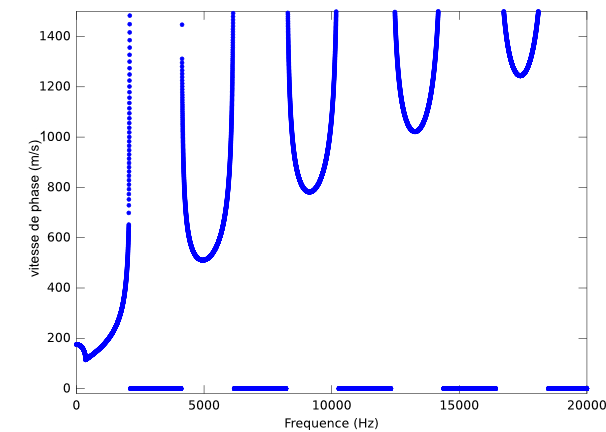
\includegraphics[scale = 0.4]{./figures/courbe_dispersion2.png}
\caption*{\scriptsize Courbe de dispersion pour une corde lestée par des poids disposés régulièrement.}
\end{figure}
\end{frame} 

%%%%%%%%%%%%%%%%%%%%%%%%%%%%%%%%%%%%%%%%%%%%%%%%%%%%%%
%%%%%%%%%%%%%%%%%%%%%%%%%%%%%%%%%%%%%%%%%%%%%%%%%%%%%%
\begin{frame}{Impédance d'entrée}
\begin{minipage}[t]{0.49\textwidth}
~\\
	\begin{equation*}
		\begin{pmatrix} T_{11} & T_{12}\\ T_{21} & T_{22} \end{pmatrix}^{N}\qquad \Rightarrow 
	\end{equation*}
\end{minipage}
\begin{minipage}[t]{0.49\textwidth}
	\begin{figure}
		\flushleft
		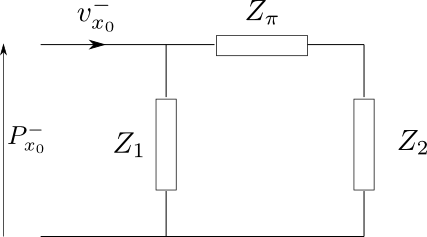
\includegraphics[scale=0.3]{./figures/schema_elec_impedance.png}
	\end{figure}
\end{minipage}
\begin{figure}[!h]\centering
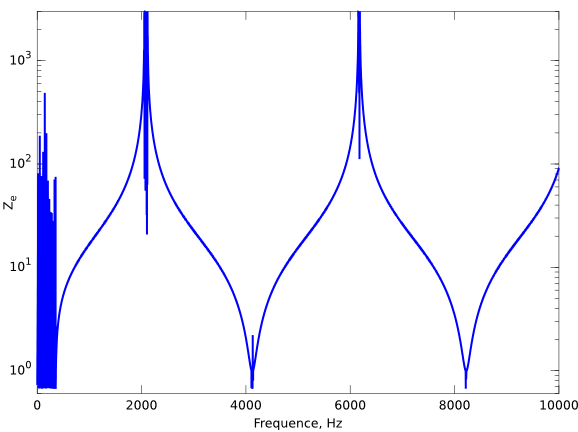
\includegraphics[scale = 0.35]{./figures/impedance_entree.png}
\caption*{\scriptsize Impédance d'entrée de la corde lestée pour une impédance de sortie infinie (N = 33).}
\end{figure}

\end{frame}

%%%%%%%%%%%%%%%%%%%%%%%%%%%%%%%%%%%%%%%%%%%%%%%%%%%%%%
%%%%%%%%%%%%%%%%%%%%%%%%%%%%%%%%%%%%%%%%%%%%%%%%%%%%%%
\begin{frame}{Protocole expérimental}
Schéma du banc de mesure:
\begin{figure}[!h]\centering
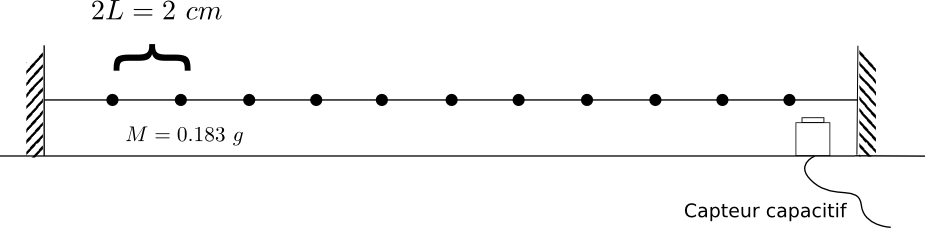
\includegraphics[scale=0.4]{./figures/schema_cordel_sans_tension.png}
\caption*{ \scriptsize Schéma du montage expérimental.}
\label{schema_cordel}
\end{figure}

Caractéristiques de la corde:
\begin{itemize}
\item Masse linéique de la corde (mesurée): $\mu = 0.63 ~g/m$
\item Longueur de la corde : $l=68 ~cm$
\end{itemize}

\end{frame}

%%%%%%%%%%%%%%%%%%%%%%%%%%%%%%%%%%%%%%%%%%%%%%%%%%%%%%
%%%%%%%%%%%%%%%%%%%%%%%%%%%%%%%%%%%%%%%%%%%%%%%%%%%%%%
\subsection{Résultats expérimentaux}
\begin{frame}{Résultats expérimentaux}

\begin{figure}[!h]\centering
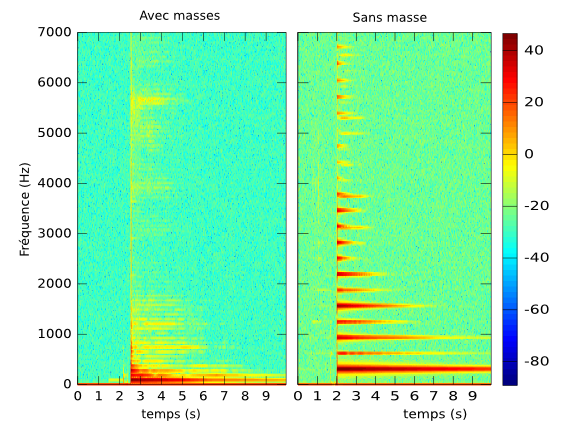
\includegraphics[scale=0.45]{./figures/spectrogram_nue.png}
\caption*{\scriptsize Spectrogramme de l'énergie dans la corde avec et sans masses.}
\end{figure} 

\end{frame}

%%%%%%%%%%%%%%%%%%%%%%%%%%%%%%%%%%%%%%%%%%%%%%%%%%%%%%
%%%%%%%%%%%%%%%%%%%%%%%%%%%%%%%%%%%%%%%%%%%%%%%%%%%%%%
\section{Conclusion}
\begin{frame}{Conclusion}
Divers manières d'obtenir une onde dispersive ont donc été vues :

\begin{itemize}
\item Dans un guide d'onde, la dispersion est liée à la prise en compte de l'impédance des parois.
\bigskip
\item Dans une poutre, le moment de torsion fait apparaître une dérivée 4\textsuperscript{ème} dans l'équation de propagation de l'onde.
\bigskip
\item Enfin, pour la corde lestée, la périodicité du réseau engendre la non-propagation pour des bandes de fréquences et influe sur la célérité des ondes dont la fréquence avoisine ces bandes.

\end{itemize}


\end{frame}

%%%%%%%%%%%%%%%%%%%%%%%%%%%%%%%%%%%%%%%%%%%%%%%%%%%%%%
%%%%%%%%%%%%%%%%%%%%%%%%%%%%%%%%%%%%%%%%%%%%%%%%%%%%%%
\begin{frame}{Bibliographies}
\indent GUYADER, Jean-Louis. Vibrations des milieux continus. Hermes Science Publications, 2002 \\~\\
\indent DALMONT, Jean-Pierre. Guide des Guides d'ondes acoustiques (version 1.4). 2010 \\ ~\\
\indent RICHOUX, Olivier. Étude de la propagation des ondes mécaniques dans un réseau unidimensionnel comportant du désordre et/ou des non-linéarités localisées. Th. doct. : Acoustique. Le Mans : université du Maine, 1999 \\~\\

\indent CASTAGNEDE, Bernard. Cours de théorie des vibrations [en ligne]. Consulté le 20/05/14. Disponible à l'adresse : \\ \url{perso.univ-lemans.fr/~bcasta/Doc Enseignement/Cours M1 Vibrations(II).pdf}


\end{frame}

\end{document}
